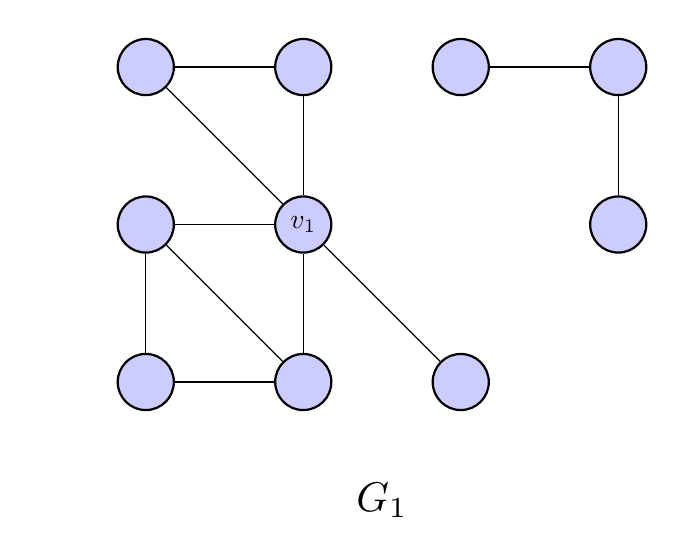
\begin{tikzpicture}[scale=1, auto=left, every node/.style={circle, fill=blue!20, draw=black, thick}]
    \node (v) at (3,2) {$v_1$};

  % Componente superior izquierda
    \node (u1) at (1,4) {\phantom{$v_1$}};
  \node (u2) at (3,4) {\phantom{$v_1$}};

  % Componente inferior izquierda
  \node (w1) at (1,2) {\phantom{$v_1$}};
  \node (w2) at (1,0) {\phantom{$v_1$}};
  \node (w3) at (3,0) {\phantom{$v_1$}};

  % Hoja inferior derecha
  \node (x1) at (5,0) {\phantom{$v_1$}};

  % Componente disjunta superior derecha
  \node (y1) at (5,4) {\phantom{$v_1$}};
  \node (y2) at (7,4) {\phantom{$v_1$}};
  \node (y3) at (7,2) {\phantom{$v_1$}};

  % Aristas
  \draw (u1) -- (u2);
  \draw (u1) -- (v);
  \draw (u2) -- (v);

  \draw (w1) -- (w2);
  \draw (w2) -- (w3);
  \draw (w1) -- (w3);
  \draw (w1) -- (v);
  \draw (w3) -- (v);

  \draw (v) -- (x1);

  \draw (y1) -- (y2);
  \draw (y2) -- (y3);

% Forzar Bounding Box idéntico en ambos diagramas
  \useasboundingbox (-0.5,-1.6) rectangle (7.5,4.5);
  % Etiqueta del grafo
  \node[draw=none, fill=none, scale=1.5] at (4,-1.5) {$G_1$};
\end{tikzpicture}
